%% ---------------------------------------------------------------------
%% Copyright 2014, Thales, IGN, Rémi Cura
%% 
%% This file is the abstract of the article
%% ---------------------------------------------------------------------


\begin{abstract} 
\begin{figure*}[t!]
	\begin{center}
		\fbox{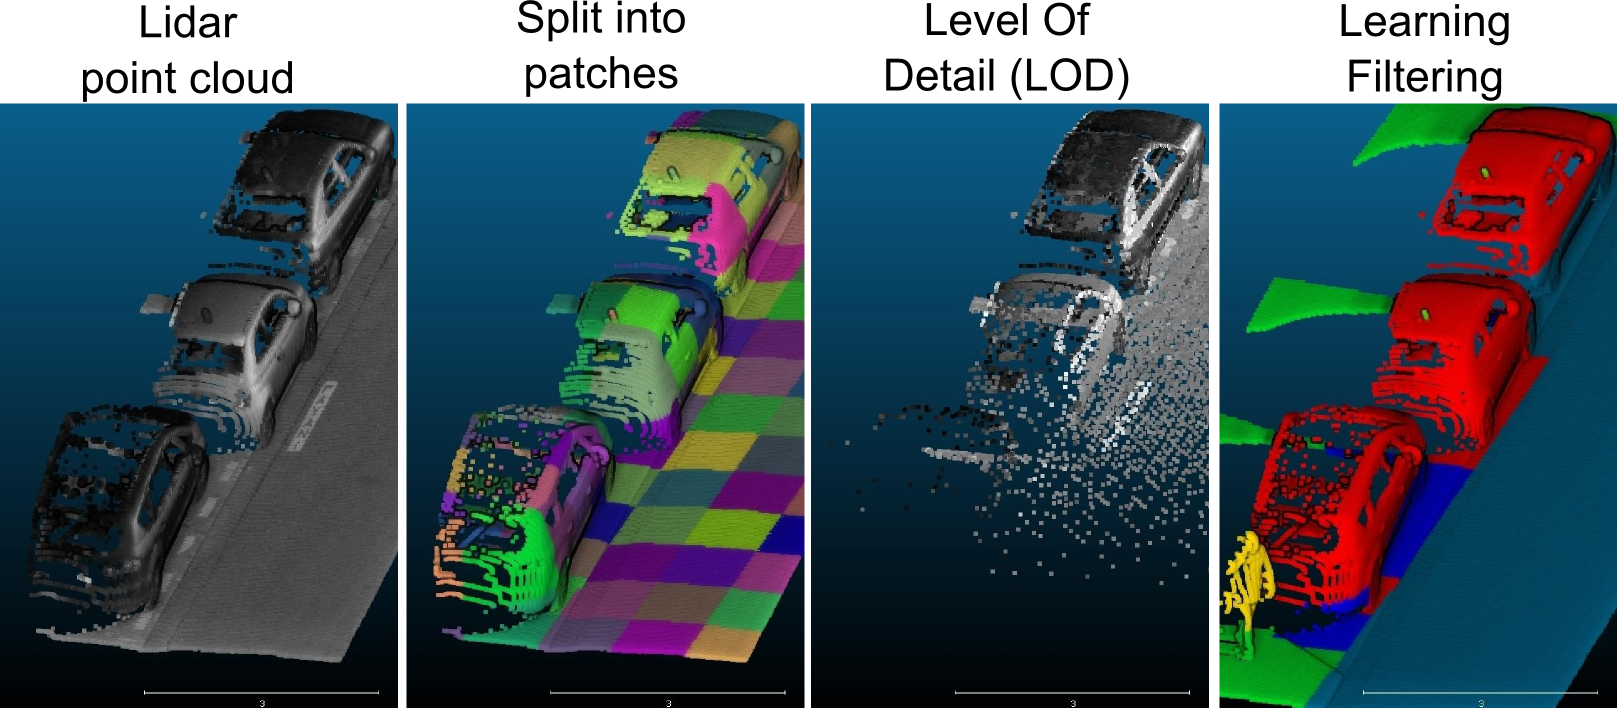
\includegraphics[width=\textwidth,keepaspectratio ]{./illustrations/banner_for_paper.png}}
		\caption{Data flow : starting from Lidar point cloud, we split it into patches, then reorder the patches to obtain free LOD (a gradient of LOD on this illustration). Lastly we use this ordering as feature for learning and efficient filtering} 
		\label{fig:banner_image}
		\end{center}
\end{figure*}
\newpage

This article introduce a new ordering for point cloud based on an octree, which allows, after a pre-computing phase to effortlessly get a representative geometric level of details of a point cloud, and even use the information as a crude classifier.

%sum um eachparts with 1-2 lines
\end{abstract}
